% !TeX spellcheck = de_DE
% !TeX root = kristallographie_skript.tex
\begin{sheet}

\begin{problem}
Schaue dir die Bilder, gedacht als 2D Kristalle, auf den folgenden Seiten an.

Bestimme
\begin{subproblem}
möglichst viele wesentlich verschiedene Symmetrien
\end{subproblem}

\begin{subproblem}
einige mögliche Basiszellen und elementare Basiszellen
\end{subproblem}

von so vielen Kristallen wie du Lust hast.
\end{problem}

\begin{problem}[difficulty={fortgeschritten}]
Das Prinzip, mit dem wir die Operation von $\Aut(\Lambda)$ auf einem 3-Torus konstruiert haben, lässt sich wie folgt abstrahieren und verallgemeinern:

Gegeben eine Gruppe $G$, einen Normalteiler $N\unlhd G$ und eine Operation von $G$ auf $\Omega$, dann operiert $G/N$ auf dem Bahnenraum $\Omega/N$ wie folgt:
\[{^{gN} B} := {^g B} := \Set{{^g \omega} | \omega\in B}\]
\begin{subproblem}[difficulty={einfach}]
Man zeige, dass dies wohldefiniert ist, d.h.
\[\forall g,h\in G, B\in\Omega/N: gN=hN \implies {^g B} = {^h B}\]
\end{subproblem}
\begin{subproblem}[difficulty={mittel}]
Man überlege sich, dass dies genau unsere Konstruktion mit dem 3-Torus ergibt, wenn wir $G=\Aut(\Lambda)$ auf $\Omega=\IR^3$ operieren lassen und $N=\mathcal{T}$ betrachten. Hinweis: Man überlege sich zuerst, wieso der 3-Torus genau $\IR^3 / \mathcal{T}$ ist.
\end{subproblem}
\end{problem}

\begin{problem}[difficulty={leicht bis mittel}]
Finde zu jedem der sieben Gittersysteme ein Translationsgitter, das in dieses Gittersystem fällt.
\end{problem}

\begin{problem}
	Andrea und Johannes haben Polyeder mitgebracht. 
	\begin{subproblem}
		Bestimme das Hermann-Mauguin-Symbol für einige Polyeder. Schreibe das Symbol auf ein Stück Papier und lege es zusammengefaltet in die Tischmitte.
	\end{subproblem}
	\begin{subproblem}
		In der Tischmitte sollten einige Zettel Papier liegen. Nimm dir einige (aber nicht die eigenen) und ordne den darauf notierten Hermann-Mauguin-Symbolen ihr jeweiliges Gittersystem zu.
	\end{subproblem}
	\begin{subproblem}[difficulty={mittel}]
		Bestimme die Tracht der Kristalle, die durch von dir die gezogenen Hermann-Mauguin-Symbole beschrieben werden.
	\end{subproblem}
	
\end{problem}
\begin{problem}[difficulty={sehr leicht}]
	Lilly hat einige Basiszellen auf ihrem Laptop mitgebracht, schaue sie dir an.
\end{problem}

\includepdf[pages=3-8, nup=1x2,angle=90]{../Übungen/Aufgabenblatt01_1}
\includepdf[pages=2-5, nup=1x2,angle=90]{../Übungen/Aufgabenblatt01_2}

\begin{problem}
	Gegeben (im Anschluss an den Bildern der 2D-Kristalle) ist eine Projektion einer Elementarzelle eines Kristalls auf die Ebene aufgespannt durch die ersten zwei Basisvektoren $a,b$. Die Position eines Atoms ist durch einen grün schraffierten Kreis gekennzeichnet. Einige \emph{mögliche} Atompositionen sind zur Unterstützung mit $A$ bis $S$ benannt.
	\begin{subproblem}
	Zu welchem Gittersystem gehört der abgebildete Kristall?
	\end{subproblem}
	\begin{subproblem}
	Was ist das Hermann-Mauguin-Symbol dieser Raumgruppe?
	\end{subproblem}
	\begin{subproblem}
	Welche der Positionen $A$ bis $S$ sind die Positionen der zum gegebenen Atom symmetrieäquivalenten Atome?
	
	Bemerkung: Wenn eine Symmetrieoperation eine Position außerhalb der gegebenen Elementarzelle erzeugt, bedenke, dass man diese stets durch ein ganzzahliges Vielfaches eines oder mehrerer Basisvektoren in die Elementarzelle zurücktransferieren kann.
	\end{subproblem}
	
	\begin{subproblem}
	Was sind die Höhen der so gefundenen Atome in der Elementarzelle, wenn sich das gegebene Atom auf der Höhe $+z$ befindet?
	\end{subproblem}
\begin{figure}
\includepdf[pages=2, offset=0 -270]{../Übungen/Aufgabenblatt07}
\end{figure}

\end{problem}

\end{sheet}